%% USPSC-Cap2-Desenvolvimento.tex 

% ---
% Este capítulo, utilizado por diferentes exemplos do abnTeX2, ilustra o uso de
% comandos do abnTeX2 e de LaTeX.
% ---

\chapter{Materials and Methods}\label{ch:mat}

\section{Core data and scripts}\label{sec:data}\label{scripts}
Email list messages were obtained from
the Gmane email archive, which consists of more than $20,000$
email lists (discussion groups) and more than $130\times 10^6$ messages~\cite{Gmanewikipedia}. These lists cover a variety of topics, mostly technology-related. The archive can be described as a corpus along with message metadata, including sent time, place, sender name, and sender email address.
The usage of the Gmane database in scientific research is reported in studies of isolated lists and of lexical innovations~\cite{Gmane2,bird}. 

We observed various email lists and selected five of them together with data from Twitter, Facebook and Participabr for a thorough analysis,
from which general properties can be inferred. These lists are as follows:

\begin{itemize}
\item Linux Audio Users list\footnote{gmane.linux.audio.users is list ID in Gmane.},with participants from different countries with artistic and technological interests. English is the prevailing language. Abbreviated as LAU from now on.

\item Linux Audio Developers list\footnote{gmane.linux.audio.devel is list ID in Gmane.}, with participants from different countries; a more technical and less active version of LAU. English is the prevailing language. Abbreviated as LAD from now on.

\item Developer's list for the standard C++ library\footnote{gmane.comp.gcc.libstdc++.devel is list ID in Gmane.}, with computer programmers from different countries. English is the prevailing language. Abbreviated as CPP from now on.
\item List of the MetaReciclagem project\footnote{gmane.politics.organizations.metareciclagem is list ID in Gmane.}, a Brazilian email list for digital culture. 	Portuguese is the prevailing language, although some messages are written in Spanish and English. Abbreviated as MET from now on.
\item List for de discussion of the election reform\footnote{gmane.politics.election-methods is list ID in Gmane.}. English is the prevailing language. Abbreviated ELE from now on.
\end{itemize} 

The first 20,000 messages of each list were considered, with basic attributes of total timespan, authors, threads and missing messages indicated in Table~\ref{tab:genLists}. We considered 140 additional email lists to report on the interdependence between the number of participants and the number of discussion threads. Furthermore, 12 networks from Facebook (8), Twitter (2) and Participabr (2) were scrutinized, and their analysis is given in the Supporting Information document for the purpose of testing the generality of the results.
We systematicaly used 18 lists for taking text-related measures.

 
\begin{table}
\centering
\caption{Columns $date_1$ and $date_M$ have dates of first and last messages from the 20,000 messages considered in each email list.
$N$ is the number of participants (number of different email addresses),
$\Gamma$ is the number of discussion threads (count of messages without antecedent),
$\overline{M}$ is the number of messages missing in the 20,000 collection
($100\frac{23}{20000}=0.115$ percent in the worst case).
}
\label{tab:genLists}
\begin{tabular}{|l|c|c|c|c|c|}\hline
list & $date_1$ & $date_{M}$    & $N$  & $\Gamma$ & $\overline{M}$ \\\hline
LAU & 2003-06-29  & 2005-07-23  & 1147  & 3374  & 5 \\\hline
LAD & 2003-07-03  & 2009-10-07  & 1232  & 3114  & 4 \\\hline
MET & 2005-08-01  & 2008-03-07  & 477  & 4607  & 23 \\\hline
CPP & 2002-03-12  & 2009-08-25  & 1036  & 4506  & 7 \\\hline
ELE & 2002-03-18  & 2011-08-31  & 302  & 6070  & 54 \\\hline

\end{tabular}
\begin{flushleft}
		Source: Prepared by the authors.\
\end{flushleft}
\end{table} 

\subsection{Linked Open Social Database for scientific benchmarking}
Beyond core data used to derive topological and text related results,
we provided a database for scientific benchmarking and to derive further results in our research.
The data used here were obtained from Facebook, Twitter, IRC, Email lists and the
detached instances of ParticipaBR, AA and Cidade Democr\'atica.
These were represented as linked data to homonenize access,
complying with current best practices and facilitationg analyzes which integrate third
party and provided instances. 
 
Data was gathered from:
\begin{itemize}
	\item public APIs (Twitter, Email);
	\item public logs (IRC and AA);
	\item Netvizz software~\cite{netvizz} and subsequent donation by users (Facebook);
	\item donation by system administrators (AA, ParticipaBR, Cidade Democr\'atica).
\end{itemize}

This section introduces the underlying data in a very concise fashion.
Further information is available in the Appendix~\ref{ap:losd} and in an article~\cite{losd}.
 
\subsubsection{Snapshots}
Of central importance to the provided database is the concept of a snapshot.
A snapshot is herein a set of data gathered together,
at a contiguous time span.
For example: the first 20 thousand email messages of an email list
comprises a snapshot; the tweets from the MAMA music event are a
snapshot; the friendship, interaction and posts structures of a facebook
group, prospected at the same time, are a snapshot.

\subsubsection{Facebook data}
Friendship ego networks (networks whose constituents are friends of a user)
were donated from individual users in 2013 and 2014.
Friendship and interaction networks from groups were gathered from
groups where the author was a participant.
Additionally, some groups have post texts along some metadata, such as
the number of likes.

\subsubsection{Twitter data}
Tweets were gathered through the Twitter streaming public API.
Each snapshot is unified by a distinct hashtag.
Edges are canonically yield by retweets but replies and user mentions
are also kept in the database.

\subsubsection{IRC data}
Public IRC logs were used to render IRC snapshots.
The database has records of users to which the message is directed or
mentions.

\subsubsection{Email data}
Email snapshots refer to individual email lists.
All messages were obtained from the Gmane public email database~\cite{gmane}.
Each message has the original text and the text without some of the lines
from previous messages or that are software code.
Most importantly, each message instance holds the ID of the message it is
a reply to, if any.

\subsubsection{ParticipaBR data}
The ParticipaBR is a Brazilian federal platform for social participation.
Texts are derived from blog posts and networks are derived from
friendship and interaction criteria.

\subsubsection{Cidade Democr\'atica data}
Cidade Democr\'atica is a Brazilian civil society social participation portal.
Data gathered is complex with many types of instances and no intuitive criteria
for deriving networks, such as friendships or replies.

\subsubsection{AA data}
The Algorithmic Autoregulation~\cite{aa} is a software development
methodology based on testifying and sharing ongoing work.
The data was gathered from different versions of the system and from an IRC
log. 

\subsection{Availability}
The data and scripts used to derive the results, figures and tables are publicly available. Email messages are downloadable from the Gmane public database~\cite{Gmanewikipedia}.
Data annotated from Facebook and Twitter are in a public repository~\cite{fbtwData}.
Data from Participabr was used from the linked data/semantic web RDF triples~\cite{opa}, available in~\cite{datahub}.
Computer scripts are delivered through public domain Python PyPI packages and open Git repositories~\cite{gmanePack}.
This open approach to both data and scripts reinforces the scientific aspect of the contribution~\cite{openSci} and mitigates ethical and moral issues involved in researching systems constituted of human individuals~\cite{anPhy,ccs15}.
 
\section{Methods}\label{sec:carac}
%The networks were characterized with: 1) statistics of activity along time, in scales from seconds to years; 2) dispersion of basic topological metrics; 3) sectioning of the networks in hubs, intermediary and periphery; 4) iterative visualization, sonification and data inspection.
%These procedures are described below.

\subsection{Temporal activity statistics}\label{sec:mtime}
Messages were counted over time as histograms in the scales of seconds,
minutes, hours, days of the week, days of the month, and months of the year.
Most standard measures of location and dispersion, e.g. the usual mean and
standard deviation, hold little meaning in a compact Riemannian manifold,
such as the recurrent time periods that we are interested in.
Similar measures were taken using circular statistics~\cite{directionalStats},
in which each measurement $t$ is represented as a unit complex number,
$z=e^{i\theta}=\cos(\theta)+i\sin(\theta)$, where $\theta=t\frac{2\pi}{T}$,
and $T$ is the period in which the counting is repeated.
For example, $\theta=12\frac{2\pi}{24}=\pi$ for a message sent at $t=12h$ and given $T=24h$ for days.
The moments $m_n$, lengths of moments $R_n$, mean angles $\theta_\mu$, and rescaled mean angles $\theta_\mu'$ are defined as:

\begin{align}\label{eq:cmom}
m_n&=\frac{1}{N}\sum_{i=1}^N z_i^n \nonumber\\
R_n&=|m_n|\\
\theta_\mu&=Arg(m_1) \nonumber \\
\theta_\mu'&=\frac{T}{2\pi} \theta_\mu \nonumber
\end{align}

$\theta_\mu'$ is used as the measure of location.
Dispersion is measured using the circular variance $Var(z)$,
the circular standard deviation $S(z)$, and the circular dispersion $\delta(z)$:

\begin{align}\label{eq:cmd}
Var(z)&=1 - R_1 \nonumber\\
S(z)&= \sqrt{-2\ln(R_1)}\\
\delta(z)&=\frac{1-R_2}{2 R_1^2} \nonumber
\end{align}

\noindent
Also, the ratio $r=\frac{b_l}{b_h}$ between the lowest $b_l$ and the highest $b_h$ incidences on the histograms 
served as a further clue of how close the distribution was to being uniform. As expected, a positive correlation was found in all $r, Var(z)$, $S(z)$ and $\delta(z)$ dispersion measures,
which can be noticed in Section~\ref*{si:circ}.
The circular dispersion $\delta(z)$ was found more sensitive and therefore preferred in the discussion of results.

\subsection{Interaction networks}\label{intNet}
Edges in interaction networks can be modeled both as weighted or unweighted, as directed or undirected~\cite{bird,newmanCommunityDirected,newmanCommunity2013}.
Networks in this thesis are directed and weighted, the most informative of the possibilities. We did not investigate directed unweighted, undirected weighted, and undirected unweighted representations of the interaction networks. 

The interaction networks were obtained as follows: a direct response from participant B to a message from participant A yields an edge from A to B, as information went from A to B. The reasoning is: if B wrote a response to a message from A, he/she read what A wrote and formulated a response, so B assimilated information from A, thus $A \rightarrow B$.
Edges in both directions are allowed. Each time an interaction occurs, the value of one is added to the edge weight. Selfloops were regarded as non-informative and discarded. Inverting edge direction yields the status network: B read the message and considered what A wrote worth responding, giving status to A, thus $B\rightarrow A$. This thesis considers by convention the information network as described above ($A\rightarrow B$) and depicted in Figure~\ref{formationNetwork}. These interaction networks are reported in the literature as exhibiting scale-free and small-world properties, as expected for a number of social networks~\cite{bird,newmanBook}.

\begin{figure}[!h]
\centering
\caption{The formation of interaction networks from exchanged messages. Each vertex represents a participant. A reply message from author B to a message from author A is regarded as evidence that B received information from A and yields a directed edge. 	Multiple messages add ``weight'' to a directed edge. Further details are given in Section~\ref{intNet}.}
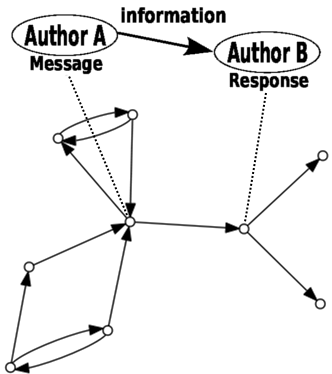
\includegraphics[width=0.5\textwidth]{figs/criaRede3_}
\label{formationNetwork}
\begin{flushleft}
		Source: Prepared by the authors.\
\end{flushleft}
\end{figure}

%Edges can be created from all antecedent message authors on the message-response thread to each message author.
%We only linked the immediate antecedent to the new message author, both for simplicity and because in adding two edges, $x\rightarrow y$ and $y\rightarrow z$, there is also a weaker connection between $x$ and $z$. Potential interpretations for this weaker connection are: double length, half weight or with one more ``obstacles''. This suggests the adequacy of centrality measurements to account for the connectivity of a node with all other nodes, such as betweenness centrality, eigenvector centrality and accessibility~\cite{luMeasures,access}.

\subsection{Topological metrics}\label{measures}

The topology of the networks was characterized 
from a small selection of the most basic 
and fundamental measurements for each vertex~\cite{newmanBook},
as introduced in Section~\ref{se:intMea}.
The betweenness centrality index was computed for weighted digraphs as specified in~\cite{faster}.

The non-standard metrics below were formulated to capture symmetries in the activity of participants:

\begin{itemize}
\item Asymmetry of vertex $i$: $asy_i=\frac{k_i^{in}-k_i^{out}}{k_i}$.
\item Average asymmetry of edges at vertex $i$:\\ $\mu_i^{asy}=\frac{\sum_{j\in J_i} e_{ji}-e_{ij}}{|J_i|}$, where $e_{ij}$ is 1 if there is an edge from $i$ to $j$, and $0$ otherwise, and $J_i$ is the set of neighbors of vertex $i$.
\item Standard deviation of asymmetry of edges:\\ $\sigma_i^{asy}=\sqrt{\frac{\sum_{j\in J_i}[\mu^{asy}_i -(e_{ji}-e_{ij}) ]^2  }{|J_i|}  }$.
\item Disequilibrium: $dis_i=\frac{s_i^{in}-s_i^{out}}{s_i}$.
\item Average disequilibrium of edges:\\ $\mu_i^{dis}=\frac{\sum_{j \in J_i}\frac{w_{ji}-w_{ij}}{w_{ji}+w_{ij}}}{|J_i|}$, where $w_{xy}$ is the weight of edge $x\rightarrow y$ and zero if there is no such edge.
\item Standard deviation of disequilibrium of edges: $\sigma_i^{dis}=\sqrt{\frac{\sum_{j\in J_i}\left[\mu^{dis}_i-\frac{w_{ji}-w_{ij}}{w_{ji}+w_{ij}}\right]^2}{|J_i|}}$.
\end{itemize}

Standard metrics are used for the Erd\"os sectioning (described in the next section).
Both standard and non-standard metrics are used
for performing principal component analysis (PCA) (as described in Section~\ref{sec:pca}).


\subsection{Erd\"os sectioning}\label{sectioning}
It is often useful to think of vertices as hubs, peripheral and intermediary. We have therefore derived the peripheral, intermediary and hub sectors of an empirical network from the comparison against an Erd\"os-R\'enyi network with the same number of edges and vertices,
as depicted in Figure~\ref{fig:setores}. We refer to this procedure as \emph{Erd\"os sectioning}, with the resulting sectors being named as \emph{Erd\"os sectors}. The Erd\"os sectioning was recognized as a theoretical possibility by M. O. Jackson in his video lectures~\cite{3setores}, but to our knowledge it has not as yet been applied to empirical data.

The degree distribution $\widetilde{P}(k)$ of a real network with a scale-free profile $\mathcal{N}_f(N,z)$ with $N$ vertices and $z$ edges has less
average degree nodes than the distribution $P(k)$ of an Erd\"os-R\'enyi
network with the same number of vertices and edges. Indeed, we define in this work the intermediary sector of a network to be the set of all the nodes whose degree is less abundant in the real network than on the Erd\"os-R\'enyi model:

\begin{equation}\label{criterio}
\widetilde{P}(k)<P(k) \Rightarrow \text{k is intermediary degree}
\end{equation}

If $\mathcal{N}_f(N,z)$ is directed and has no self-loops, the probability of the existence
of an edge between two arbitrary vertices is $p_e=\frac{z}{N(N-1)}$.
A vertex in the ideal Erd\"os-R\'enyi digraph with the same number of vertices and edges, and thus the same probability $p_e$ for the presence of an edge, will have degree $k$ with probability

\begin{equation}
P(k)=\binom{2(N-1)}{k}p_e^k(1-p_e)^{2(N-1)-k}
\end{equation}

The lower degree fat tail corresponds to the border vertices, i.e. the peripheral sector or periphery where $\widetilde{P}(k)>P(k)$ and $k$ is lower than any value of $k$ in the intermediary sector.
The higher degree fat tail is the hubs sector, i.e. $\widetilde{P}(k)>P(k)$ and $k$ is higher than any value of $k$ in the intermediary sector. The reasoning for this classification is as follows: vertices so connected that they are virtually nonexistent in the Erd\"os-R\'enyi model, are coherently associated to the hubs sector.
Vertices with very few connections, which are way more abundant than expected in the Erd\"os-R\'enyi model,
are assigned to the periphery.
Vertices with degree values predicted as the most abundant in the Erd\"os-R\'enyi model,
near the average, and less frequent in the real network, are classified as intermediary.

\clearpage
\begin{figure}[!h]
\centering
\caption{Classification of vertices by comparing degree
distributions~\cite{3setores}.
The binomial distribution of the Erd\"os-R\'enyi network model exhibits more intermediary vertices, while a scale-free network, associated with the power-law distribution, has more peripheral and hub vertices. The sector borders are defined with respect to the intersections of the distributions. Characteristic degrees are in the compact intervals: $[0,k_L]$, $(k_L,k_R]$, $(k_R,k_{max}]$ for the periphery, intermediary and hub sectors, the ``Erd\"os sectors''.
The connectivity distribution of empirical interaction networks, e.g. derived from email lists, can be sectioned by comparison against the associated binomial distribution with the same number of vertices and edges. In this figure, a snapshot of 1000 messages from CPP list yields the degree distribution of an interaction network of 98 nodes and 235 edges. A thorough explanation of the method is provided in Section~\ref{sectioning}.}
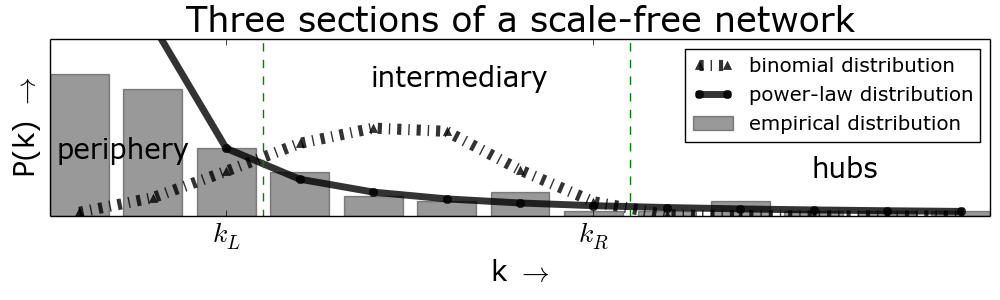
\includegraphics[width=\textwidth]{figs/fser__}
\label{fig:setores}
\begin{flushleft}
		Source: Prepared by the authors.\
\end{flushleft}
\end{figure}

To ensure statistical validity of the histograms, bins can be chosen to contain at least $\eta$ vertices of the real network.
The range $\Delta$ of incident values of degree $k$ should be partitioned in $m$ parts $\Delta=\cup_{i=1}^m \Delta_i$,
with $\Delta_i\cap \Delta_j=\emptyset \; \forall\; i \neq j$ and:
%\begin{equation}
%\begin{split}
\begin{align}
\Delta_i =\Biggl\{ k\;\; & | & \overline{\Delta}_{i-1}< &\, k\leq l \text{ and }\;\;\;\;\;\;\;\;\;\;\;\;\nonumber\\
                         & \Biggl[ \Bigl[ & N - \sum_{k=0}^{\overline{\Delta}_{i-1}} & \eta_k< \eta \text{ and } l = \overline{\Delta} \Bigr] \text{ or }\\
&	\Bigl[ & \sum_{k=\overline{\Delta}_{i-1}+1}^l &  \eta_k \geq \eta \text{ and }\;\;\;\;\;\;\nonumber\\
& \Bigl( &\sum_{k=\overline{\Delta}_{i-1}+1}^{l-1} &  \eta_k < \eta \text{ or }   l=\overline{\Delta}_{i-1}+1 \Bigr) \;\Bigr] \Biggr] \Biggr\}\nonumber
\end{align}
%\end{split}
%\end{equation}

\noindent where $\eta_k$ is the number of vertices with degree $k$,
while $\overline{\Delta}_{(i)}=max(\Delta_{(i)})$, and $\overline{\Delta}_{0}=-1$.
% and $\overline{\Delta}_{i}<l\leq max(\Delta)$.
Equation~\ref{criterio} can now be written in the form:

\begin{equation}\label{criterio2}
\begin{split}
\sum_{x=min(\Delta_i)}^{\overline{\Delta}_i} \widetilde{P}(x) < \sum_{x=min(\Delta_i)}^{\overline{\Delta}_i} P(x) \Leftrightarrow \\
\Leftrightarrow \Delta_i \text{ spans intermediary degree values.}
\end{split}
\end{equation}

If the strength $s$ is used for comparison of the real network against the Erd\"os-R\'enyi model,
$P$ remains the same, but $P(\kappa_i)$ with $\kappa_i=\frac{s_i}{\overline{w}}$ should be used, where $\overline{w}=2\frac{z}{\sum_is_i}$ is the average weight of an edge and $s_i$ is the strength of vertex $i$. For in and out degrees ($k^{in}$, $k^{out}$), the real network should be compared against
\begin{equation}
\hat{P}(k^{way})=\binom{N-1}{k^{way}}p_e^k(1-p_e)^{N-1-k^{way}},
\end{equation}

\noindent where \emph{way} can be \emph{in} or \emph{out}. In and out strengths ($s^{in}$, $s^{out}$) are divided by $\overline{w}$ and compared also using $\hat{P}$. Note that $p_e$ remains the same, as each edge yields an incoming (or outgoing) edge, and there are at most $N(N-1)$ incoming (or outgoing) edges, thus $p_e=\frac{z}{N(N-1)}$, as with the total degree.

In other words, let $\gamma$ and $\phi$ be integers in the intervals $1 \leq \gamma \leq 6$, $1 \leq \phi \leq 3$, and each of the basic six Erd\"os sectioning possibilities $\{E_{\gamma}\}$ have three Erd\"os sectors $E_{\gamma}= \{e_{\gamma, \phi} \}$ defined as

\begin{alignat}{3}\label{eq:part}
e_{\gamma,1}&=\{\;i\;|\;\overline{k}_{\gamma,L}\geq&&\overline{k}_{\gamma,i}\} \nonumber \\
e_{\gamma,2}&=\{\;i\;|\;\overline{k}_{\gamma,L}<\;&&\overline{k}_{\gamma,i}\leq\overline{k}_{\gamma,R}\} \\ 
e_{\gamma,3}&=\{\;i\;|\;&&\overline{k}_{\gamma,i}>\overline{k}_{\gamma,R}\} \nonumber,
\end{alignat}

\noindent where $\{\overline{k}_{\gamma,i}\}$ is

\begin{equation}
\begin{split}
\overline{k}_{1,i}&=k_i \\
\overline{k}_{2,i}&=k_i^{in} \\
\overline{k}_{3,i}&=k_i^{out} \\
\overline{k}_{4,i}&=\frac{s_i}{\overline{w}} \\
\overline{k}_{5,i}&=\frac{s_i^{in}}{\overline{w}} \\
\overline{k}_{6,i}&=\frac{s_i^{out}}{\overline{w}}
\end{split}
\end{equation}

\noindent and both $\overline{k}_{\gamma,L}$ and $\overline{k}_{\gamma,R}$ are found using $P(\overline{k})$ or $\hat{P}(\overline{k})$ as described above and illustrated in Figure~\ref{fig:setores}.

Since different metrics can be used to identify the three types of vertices, more than one metric can be used simultaneously, which is convenient when analysing small networks,
such as the cases where only 50 messages are considered in Section~\ref*{si:frac}.
%For example, a very stringent criterion can be used, according to which a vertex is only regarded as pertaining to a sector if it is so for all the metrics.
After a careful consideration of possible combinations, these were reduced to six:

\begin{itemize}
\item Exclusivist criterion $C_1$:  vertices are only classified if the class is the same according to all metrics. In this case, vertices classified do not usually reach $N$ (or 100\%), which is indicated by a black line in Figure~\ref{fig:sectIL}.

\item Inclusivist criterion $C_2$: a vertex has the class given by any of the metrics. Therefore, a vertex may belong to more than one class, and the total number of memberships may exceed $N$ (or 100\%), which is indicated by a black line in Figure~\ref{fig:sectIL}.

\item Exclusivist cascade $C_3$: vertices are only classified as hubs if they are hubs according to all metrics. Intermediary are the vertices classified either as intermediary or hubs with respect to all metrics. The remaining vertices are regarded as peripheral.

\item Inclusivist cascade $C_4$: vertices are hubs if they are classified as such according to any of the metrics. The remaining vertices are intermediary if they belong to this category for any of the metrics. Peripheral vertices are those which are classified as such with respect to all metrics.

\item Exclusivist externals $C_5$: vertices are hubs if they are classified as such according to all the metrics. Vertices are peripheral if they are peripheral or hubs for all metrics. The remaining nodes are intermediary.

\item Inclusivist externals $C_6$: hubs are vertices classified as hubs according to any metric. The remaining vertices are peripheral if they are classified as such according to any metric. The rest of the vertices are intermediary.
\end{itemize}

Using Equations~(\ref{eq:part}), these \emph{compound criteria} $C_\delta$, with $\delta$ integer in the interval $1\leq\delta\leq6$, can be specified as:

%\begin{alignat}{3}
\begin{equation}
\begin{split}
%\begin{multline}
C_1&=\{c_{1,\phi}=\left\{i\mid i\;\in e_{\gamma,\phi}, \;\forall\; \gamma\}\right\} \\
C_2&=\{c_{2,\phi}=\left\{i\mid \exists \;\;\gamma: i \in e_{\gamma,\phi}\}\right\} \\
C_3&=\{c_{3,\phi}=\left\{i\mid i\;\in e_{\gamma,\phi'}, \;\forall\; \gamma,\;\forall\;\phi'\geq \phi\}\right\} \\
C_4&=\{c_{4,\phi}=\left\{i\mid i\;\in e_{\gamma,\phi'}, \;\forall\; \gamma,\;\forall\;\phi'\leq \phi\}\right\} \\
C_5&=\{c_{5,\phi}=\left\{i\mid i\;\in e_{\gamma,\phi'}, \;\forall\; \gamma,\right.\\
&\;\;\;\;\;\;\;\;\;\;\;\;\;\;\;\;\;\; \left.\;\forall\;(\phi'+1)\%4\leq (\phi+1)\%4\}\right\} \\
C_6&=\{c_{6,\phi}=\left\{i\mid i\;\in e_{\gamma,\phi'}, \;\forall\; \gamma,\right.\\
&\;\;\;\;\;\;\;\;\;\;\;\;\;\;\;\;\;\; \left.\;\forall\;(\phi'+1)\%4\geq (\phi+1)\%4\}\right\} \\
%\end{multline}
\end{split}
\end{equation}
%\end{alignat}

Notice that the exclusivist cascade is the same sectioning of an inclusivist cascade from periphery to hubs, but with inverted order of sectors. 
The simplification of all possible compound possibilities to the small set listed above might be formalized in strict mathematical terms, but this was considered out of the scope for current interests.




%\subsubsection{Sectioning of networks in peripheral, intermediary and hubs sectors}\label{sectioning}
\subsection{Principal Component Analysis of topological metrics}\label{sec:pca}
Principal Component Analysis (PCA) is a well documented technique~\cite{pca} and is used here to address the following questions:	1) which metrics contribute to each principal component and in what proportion;	2) how much of the dispersion is concentrated in each component;	3) which are the expected values and dispersions for these quantities over various networks.	This enables one to characterize human interaction networks in terms of the relative importance of network metrics and the way they combine.

Let $\mathbf{X}=\{X[i,j]\}$ be a matrix where each element is the value
of the metric $j$ at vertex $i$.
Let
$\mu_X [j]=\frac{\sum_i X[i,j]}{I}$ be the mean of metric $j$ over all $I$ vertices, 
$\sigma_X [j]=\sqrt{\frac{\sum_i (X[i,j]-\mu_X [j])^2}{I}}$ the standard deviation of metric $j$,
and $\mathbf{X'}=\{X'[i,j]\}=\left\{\frac{X[i,j]-\mu_X[j]}{\sigma_X[j]}\right\}$ 
the matrix with the \emph{z-score} of each metric. 
Let $\mathbf{V}=\{V[j,k]\}$ be the matrix $J\times J$ of eigenvectors
of the covariance matrix $\mathbf{C}$
of $\mathbf{X'}$, one eigenvector per column.
Each eigenvector combines the original metrics into one principal component, therefore
$V'[j,k]=100\frac{|V[j,k]|}{\sum_{j'} |V[j',k]|}$
is the percentage of the principal component $k$
that is proportional to the metric $j$.
%With $k$ eigenvectors 
%$D[k]$,
%it is enough to 
Let $\mathbf{D}=\{D[k]\}$ be the eigenvalues associated with the eigenvectors $\mathbf{V}$,
then $D'[k]=100\frac{D[k]}{\sum_{k'}D[k']}$
is the percentage of total dispersion of the system that the principal component $k$
is responsible for.
We consider, in general, the three largest eigenvalues and
the respective eigenvectors in percentages:
$\{(D'[k],\;V'[j,k])\}$.
These usually sum up between 60 and 95\% of the dispersion
and reveal patterns for a first analysis.
In particular, 
given $L$ snapshots $l$ of the interaction network,
we are interested in the mean
$\mu_{V'}[j,k]$
and the standard deviation $\sigma_{V'}[j,k]$ 
of the contribution of metric $j$ to the principal component $k$,
and the mean
$\mu_{D'}[k]$
and the standard deviation 
$\sigma_{D'}[k]$
of the contribution of the component $k$ to the dispersion
of the system:

\begin{align}\label{eq:pca}
\mu_{V'}[j,k]   &=\frac{\sum_{l=1}^L V'[j,k,l]}{L}\nonumber\\
\sigma_{V'}[j,k]&=\sqrt{\frac{\sum_{l=1}^L (\mu_{V'}-V'[j,k,l])^2}{L}}\\\nonumber
\mu_{D'}[k]&=\frac{\sum_{l=1}^L D'[k,l]}{L}\\\nonumber
\sigma_{D'}[k]&=\sqrt{\frac{\sum_{l=1}^L (\mu_{D'}-D'[k,l])^2}{L}}
\end{align}

The covariance matrix 
$\mathbf{C}$ is the correlation matrix because $\mathbf{X'}$ is normalized.
Therefore, $\mathbf{C}$ is also directly observed as a first clue for patterns
by the most simple associations:
low absolute values indicate low correlation (and a possible independence);
high values indicate positive correlation;
negative values with a high absolute value indicate negative correlation.
Notice that in this case the variable $k$ is not the degree value
but a principal component.
In the results, the principal components are numbered
according to the magnitude of associated eigenvalue and $k$ is incorporated into
the notation (e.g. PC2 for metrics of $\mu_{V'}[j,2]$).


\subsection{Evolution and audiovisualization of the networks}\label{sec:viz}
The evolution of the networks was observed within 
sequences of snapshots. In each sequence, a fixed number of messages,
i.e. the window size $ws$, was used for all snapshots.
%was considered with different shifts in the message timeline to obtain snapshots.
The snapshots were made disjoint in the message timeline, and were used to perform both PCA with topological metrics and Erd\"os sectioning.  
Figures and tables were usually inspected with 
$ws=\{50, 100, 200, 400, 500, 800, 1000, 2000, 2500, 5000, 10000\}$ messages. Variations in the number of vertices, edges
and other network characteristics, within the same window size $ws$,
are given in Section~\ref*{si:frac}. 

\subsection{The Versinus graph visualization method}
Network structures were mapped to video animations, sound and musical structures developed for this research~\cite{animacoes}.% ,galGmane,appGmane}.
Such \emph{audiovisualizations} were crucial in the initial steps and
to guide the research into the most important features of network evolution.
Versinus is a visualization method for dynamic graphs based on experimental observations.
This method received dedicated attention by recurrence of the suggestion, by fellow researchers,
to write about it.  
In visualizing a network, the method consists of creating an animation,
of a fixed-size message sliding window (e.g. 400 messages) and 
partitioning the network in two fixed-layout segments:
a sinusoid for the most connected vertexes (hubs and intermediary)
and a straight line for the less connected (peripheral).
A vertex holds the same position throughout the animation. Also,
visual cues of properties - such as color, height and width,
and rank of vertex with degree criteria - play a central role.
Numbers with individual measures for each vertex blink periodically.
Versinus differs from the few works on the visualization of dynamic
graphs because it is a simple method that has developed for practical needs and is the result of experimentations,
although a number of criteria have guided its development~\cite{Viz1,Viz2,Viz3}.

Let $\Delta$ be a fixed number of messages (e.g. $\Delta=400$).
Let also $s_{i}^{i+\Delta}$ be sets of $\Delta$ consecutive email messages along time.
A sequence $S^{\Delta,M}$ of such sets,
with the first message positioned in each the $M$ messages (e.g. $M=20000$),
can be written as: 

\begin{equation}
	S^{\Delta,M}=\{s_i^{i+\Delta}\}_{i=0}^{M-\Delta}
\end{equation}

Each set $s_i$ yields an interaction network, as described in Section~\ref{intNet}.
Each of such sequence $S^{\Delta,M}$ of sets presents stable properties,
while each participant exhibits a wide variation of characteristics.
Understanding the mechanisms of this compatibility (unstable vertices and stable network)
led to experimenting with a series of layouts and visualization techniques, from which Versinus emerged.

Taking advantage from the fact that vertices are roughly split into usual $80\%$ of peripheral, $15\%$ of intermediary and $5\%$ of hubs,
hubs are laid on the first half of a sinusoid,
intermediary on the second half,
and peripheral on the straight line.
This configuration can be improved in various forms, to which Section~\ref{sec:verref} is dedicated.
Figure~\ref{fig:versinus} has an image of such a layout.
The fixed position of each vertex is defined by the overall structure,
i.e. with respect to all $M$ messages.

\begin{figure}[h!]
	\begin{center}
				    \caption{The Versinus visualization method in use. 5\% of the most connected vertexes (hubs) are on the left half-period of the sinusoid.
				    15\% of the most connected remaining vertices are on the right half-period.
				    80\% of the least connected vertices are on the straight line, above the sinusoidal shape.
				    White dots in the bottom with numbers keep track of node position in the overall degree ordering.
				    Measures blink periodically near the vertices they are related to.}
		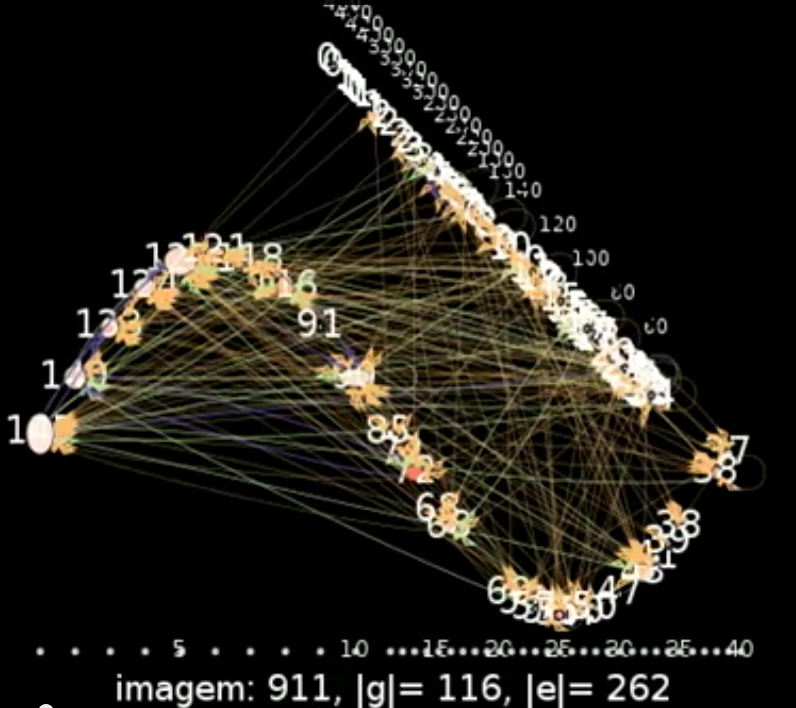
\includegraphics[scale=.45]{figs/versinus_}
					    \label{fig:versinus}
\begin{flushleft}
		Source: Prepared by the authors.\
\end{flushleft}
	\end{center}
\end{figure}


\subsection{Textual measures}
This work focuses on very simple metrics derived from texts as they have been sufficient for current interests.
Such metrics are:
\begin{itemize}
    \item Frequency of characters: letters, vowels, punctuations and uppercase letters.
    \item Number of tokens, frequency of punctuations among tokens, frequency of known words, frequency of words that have Wordnet synsets, frequency of tokens that are stopwords.
    \item Mean and standard deviation for word, token sentence and message sizes.
    \item Fraction of morphosyntactic classes, such as adverbs, adjectives, nouns and other POS (Part-Of-Speech) tags.
    \item Fraction of words in each Wordnet~\cite{wordnet} top-most hypernyms,
	    such as abstraction and physical entities for nouns or act for verbs.
    \item Mean and standard deviation of the number of Wordnet synset relations, such as holonyms and meronyms, domains, lemmas and verb groups.
\end{itemize}
% \noindent To such measures are dedicated Tables~\ref{tab:cha},~\ref{tab:tokens},~\ref{tab:sizesTokens},~\ref{tab:sizesSents},~\ref{tab:sizesMsgs},~\ref{tab:pos}.

This choice is based on: 1) the lack of such information in the literature, to the best of our knowledge; 
2) potential relations of these incidences with topological aspects, such as connectivity;
3) the interdependence of textual artifacts suggests that simple measures should reflect complex and more subtle aspects.
A preliminary study, with the complete works from the Brazilian writer Machado de Assis (in Section~\ref{ap:machado}),
made clear that these metrics vary with respect to style.

\subsubsection{About Wordnet}
In this thesis, we made use of the statistics derived from the incidence of Wordnet synsets and their characteristics.
This calls for a brief description of what is Wordnet, what is a synset and what are such characteristics:
\begin{itemize}
	\item Wordnet: a lexical database for the English language released in a BSD style license. It groups synonyms into synsets, provides a number of relations among the synsets, definitions and use examples.
	\item Synset: defined by Wordnet documentation as a set of one or more synonyms that are (somewhat) interchangeable without changing the true value of the proposition in which they occur.
	\item Synset characteristics: a synset is associated to other synsets by a number of semantic relations which differ with the POS tag attributed to them.
		Examples of such relations are yield by hyponyms and hypernyms (respectively less and more general terms), meronyms and holonyms (respectively is part of and has part), lemmas (canonical forms of a word), similar words by semantic criteria, entailments.
		Some characteristics are derived from the synset in relation to the whole Wordnet network.
		In this respect, we used only the maximum and minimum depth of the synset, which are respectively the maximum and minimum number of hypernyms from the synset to the root synset (e.g. 'thing' for nouns).
\end{itemize}

\subsubsection{Relating text and topology}\label{sec:ks}
The topological and textual measures were related by:
\begin{enumerate}
	\item textual measures in hub, intermediary and peripheral network sectors, which are delimited by topological criteria as described in Section~\ref{sectioning}.
    \item Correlation of measures of each vertex, facilitating pattern detection involving topology of interaction and language.
    \item Principal components formation derived from usual Principal Components Analysis.
\end{enumerate}

An adaptation of the Kolmogorov-Smirnov test was used to observe differences in textual content, as follows.
Let $F_{1,n}$ and $F_{2,n'}$ be two empirical distribution functions, where $n$ and $n'$ are the number of observations on each sample.
The two-sample Kolmogorov-Smirnov test rejects the null hypothesis if:
\begin{equation}\label{eq:ks}
D_{n,n'} > c(\alpha)\sqrt{\frac{n+n'}{nn'}}
\end{equation}

\noindent where $D_{n,n'}=sup_x[F_{1,n}-F_{2,n'}]$ is the Kolmogorov-Smirnov statistic
and $c(\alpha)$ is related to the significance level $\alpha$ by:

\begin{table}[H]
\centering
\begin{tabular}{|l||c|c|c|c|c|c|}\hline
$\alpha$    & 0.1  & 0.05 & 0.025 & 0.01 & 0.005 & 0.001 \\\hline
$c(\alpha)$ & 1.22 & 1.36 & 1.48  & 1.63 & 1.73  & 1.95  \\\hline
\end{tabular}
\begin{flushleft}
	Source: Wikipedia \url{https://en.wikipedia.org/wiki/Kolmogorov%E2%80%93Smirnov_test}.\
\end{flushleft}
\end{table}

We need to compare empirical distribution functions,
therefore $D_{n,n'}$ is given, as are $n$ and $n'$.
All terms in equation~\ref{eq:ks} are positive and $c(\alpha)$ can be isolated:

\begin{equation}\label{eq:ks2}
c(\alpha) < \frac{D_{n,n'}}{\sqrt{\frac{n+n'}{nn'}}} = c'
\end{equation}

When $c'$ is high, low values of $\alpha$ favor rejecting the null hypothesis.
For example, when $c'$ is greater than $\approx 1.7$, one might assume that $F_{1,n}$ and $F_{2,n'}$ differ.
We used $c'$ as a measure of how much
the distributions differ~\cite{kolm}
and for deriving hypotheses
about how different are the underlying mechanisms of generation of texts.
We made systematic measurements of the $c'$ statistic in Section~\ref{ap:ks}
which illustrate that $c'$ and $D_{n,n'}$ are useful in considering the
similarity or difference in the distributions underlying sets of samples.
A note of caution should be given here: what is a difference in distributions
might vary with context.
A $D_{n,n'}$ of only $0.0001$ will yield a very large $c'$ if $n$ and $n'$ are large enough
On the other hand, a large $D_{n,n'}$ with a small $c'$ is not a strong evidence that
the distributions differ.
Therefore, we consider both $D_{n,n'}$ and $c'$ simultaneously in our analysis.
